\section{Second Readers Writers Problem}
\subsection{Aim}
To implement the Second Readers-Writers Problem.

\subsection{Theory}
\textbf{The problem statement}: There is a shared resource which should be accessed by
multiple processes. There are two types of processes in this context: the reader and
the writer. Any number of readers can read from the shared resource simultaneously,
but only one writer can write to the shared resource. When a writer is writing data
to the resource, no other process can access the resource. A writer cannot write to
the resource if there are non zero number of readers accessing the resource at that
time. \\
\textbf{Solution}: In this solution, preference is given to the writers. This is done by
forcing every reader to lock and release the readTry mutex individually. In the case
of writers, only the first writer will lock the readTry and then all subsequent writers
can simply use the resource as it gets freed by the previous writer. The very last
writer must release the readTry semaphore, thus opening the gate for readers to try
reading.\\
The resource semaphore can be locked by both the writer and the reader in their
entry section. They are only able to do so after first locking the readTry semaphore,
which can only be done by one of them at a time.
If there are no writers wishing to get to the resource, as indicated to the reader
by the status of the readtry semaphore, then the readers will not lock the resource.
As soon as a writer shows up, it will try to set the readtry and wait for the current
reader to release the readtry.
\\
The rmutex and wmutex are used in exactly the same way as in the first read-
ers writers problem. Their sole purpose is to avoid race conditions on the readers
and writers while they are in their entry or exit sections.

\subsection{Algorithm}
\begin{verbatim}
1 semaphore resource=NULL, rmutex=NULL, wmutex=NULL, r e s=NULL;
2 readcount =0, writecount =0;
3 procedure READER
4 <ENTRY Section>
5 readTry.P()
6 rmutex.P()
7 readcount++
8 if readcount == 1 then
9 resource.P()
10 end if
11 rmutex.V()
12 readTry.V()
13 <CRITICAL Section>
14 <EXIT Section>
15 rmutex.P()
16 readcount++
17 if readcount == 0 then
18 resource.V()
19 end if
20 rmutex.V()
21 end procedure
22 procedure W RITER
23 <ENTRY Section>
24 wmutex.P() ;
25 writecount++
26 if writecount == 1 then
27 readtry.P()
28 end if
29 wmutex.V()
30 <CRITICAL Section>
31 resource.P()
32 resource.V()
33 <EXIT Section>
34 writecount--;
35 if writecount == 1 then
36 readTry.V()
37 end if
38 wmutex.V()
39 end procedure
\end{verbatim}

\subsection{Source Code}
\subsubsection{Ordinary pipe}
\begin{lstlisting}[language=C]
#include <pthread.h>
#include <semaphore.h>
#include <stdio.h>

#define NO_OF_READERS 5
#define NO_OF_WRITERS 3

// Semaphore to avoid updation while readers are active
static sem_t write_lock;

// Number of active readers and writers
static int n_reader = 0, n_writer = 0;

// Mutex lock to lock other threads from editing n_reader
// or n_writer
static pthread_mutex_t n_reader_lock, n_writer_lock, try_read;

static int data = 1000;

// Reader function
void *reader_start_routine(void *tid) {
  int thread_id = *((int *)tid);

  printf("[Reader%d]: Waiting to acquire lock for incrementing n_reader\n",
         thread_id);
  pthread_mutex_lock(&try_read);
  pthread_mutex_lock(&n_reader_lock);

  printf("[Reader%d]: Updating n_reader\n", thread_id);
  ++n_reader;
  if (n_reader == 1) {
    printf("[Reader%d]: First reader. Acquiring write lock\n", thread_id);
    sem_wait(&write_lock);
  }

  printf("[Reader%d]: Unlocking n_reader lock\n", thread_id);
  pthread_mutex_unlock(&n_reader_lock);
  pthread_mutex_unlock(&try_read);

  printf("[Reader%d]: Read value: %d\n", thread_id, data);

  printf("[Reader%d]: Waiting to acquire lock for decrementing n_reader\n",
         thread_id);
  pthread_mutex_lock(&n_reader_lock);

  printf("[Reader%d]: Updating n_reader\n", thread_id);
  --n_reader;
  if (n_reader == 0) {
    printf("[Reader%d]: No readers left. Unlocking write lock\n", thread_id);
    sem_post(&write_lock);
  }

  printf("[Reader%d]: Unlocking n_reader lock\n", thread_id);
  pthread_mutex_unlock(&n_reader_lock);
}

// Writer function
void *writer_start_routine(void *tid) {
  int thread_id = *((int *)tid);

  printf("[Writer%d]: Waiting to acquire lock for incrementing n_writer\n",
         thread_id);
  pthread_mutex_lock(&n_writer_lock);

  printf("[Writer%d]: Updating n_writer\n", thread_id);
  ++n_writer;
  if (n_writer == 1) {
    printf("[Writer%d]: First reader. Acquiring n_reader lock\n", thread_id);
    pthread_mutex_lock(&try_read);
  }

  printf("[Writer%d]: Unlocking n_writer lock\n", thread_id);
  pthread_mutex_unlock(&n_writer_lock);

  printf("[Writer%d]: Waiting for write lock\n", thread_id);
  sem_wait(&write_lock);

  printf("[Writer%d]: Write lock acquired. Incrementing value\n", thread_id);
  ++data;

  printf("[Writer%d]: Unlocking write lock\n", thread_id);
  sem_post(&write_lock);

  printf("[Writer%d]: Waiting to acquire lock for decrementing n_writer\n",
         thread_id);
  pthread_mutex_lock(&n_writer_lock);

  printf("[Writer%d]: Updating n_reader\n", thread_id);
  --n_writer;
  if (n_writer == 0) {
    printf("[Writer%d]: No writer left. Unlocking n_reader lock\n", thread_id);
    pthread_mutex_unlock(&try_read);
  }

  printf("[Writer%d]: Unlocking n_writer lock\n", thread_id);
  pthread_mutex_unlock(&n_writer_lock);
}

int main() {
  pthread_t readers[NO_OF_READERS], writers[NO_OF_WRITERS];
  int reader_ids[NO_OF_READERS], writer_ids[NO_OF_WRITERS];

  sem_init(&write_lock, 0, 1); // Initializing the semaphore
  pthread_mutex_init(&n_reader_lock, 0);
  pthread_mutex_init(&n_writer_lock, 0);

  for (int i = 0; i < NO_OF_READERS; reader_ids[i++] = i);
  for (int i = 0; i < NO_OF_WRITERS; writer_ids[i++] = i);

  for (int i = 0; i < NO_OF_READERS; i++) pthread_create(
    &readers[i], 
    NULL, 
    reader_start_routine,
    (void *)&reader_ids[i]
  );

  for (int i = 0; i < NO_OF_WRITERS; i++) pthread_create(
    &writers[i], 
    NULL, 
    writer_start_routine,
    (void *)&writer_ids[i]
  );

  for (int i = 0; i < NO_OF_READERS; i++)
    pthread_join(readers[i], NULL);
  for (int i = 0; i < NO_OF_WRITERS; i++)
    pthread_join(writers[i], NULL);

  return 0;
}
\end{lstlisting}

\begin{center}
	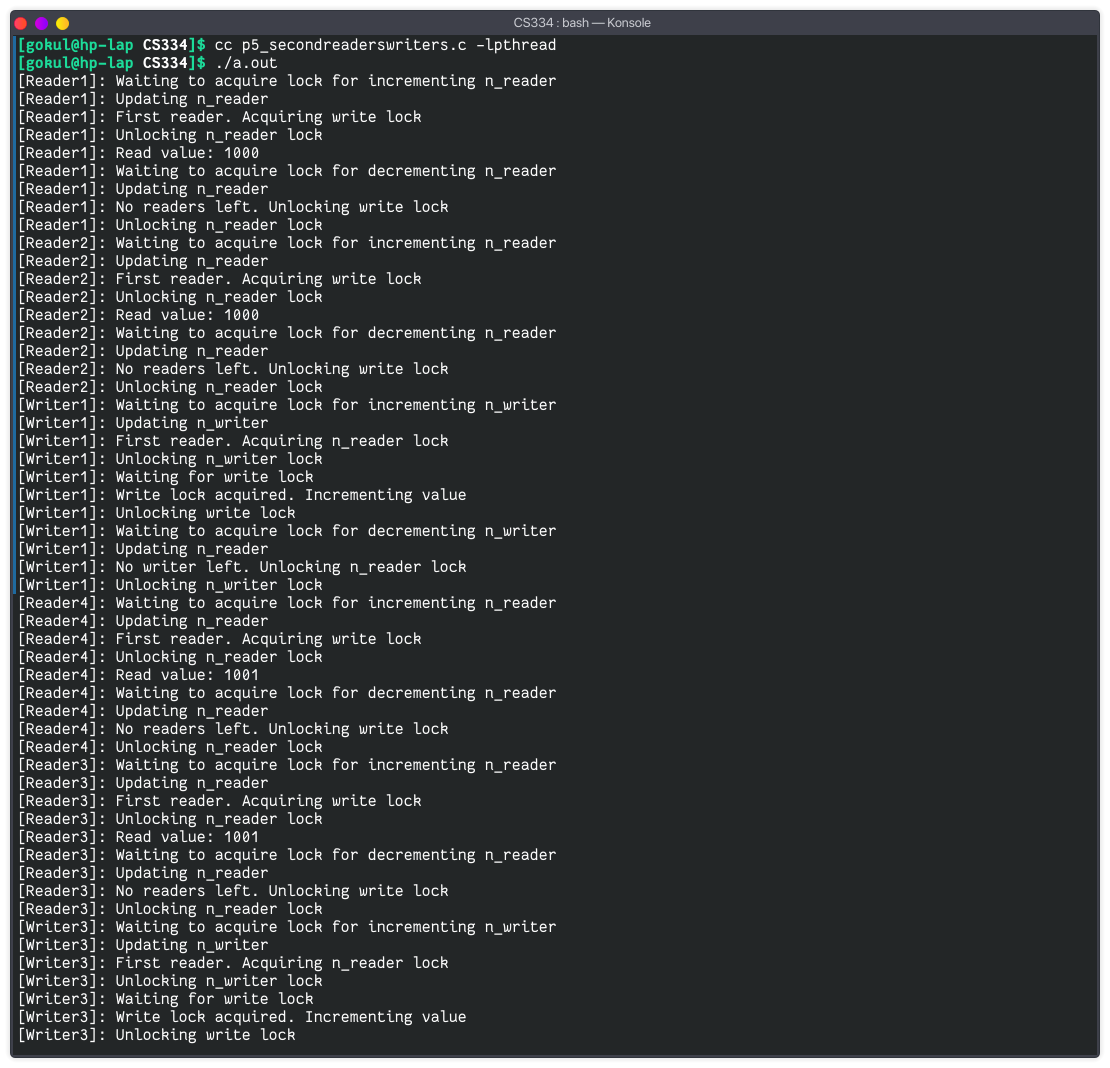
\includegraphics[width=0.90\textwidth]{img/p6/ss1.png}
	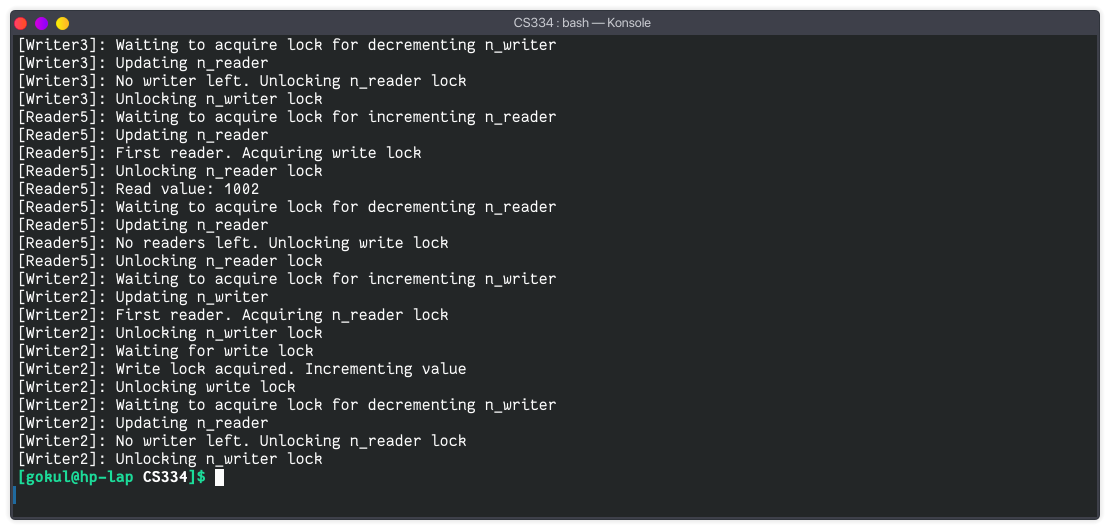
\includegraphics[width=0.90\textwidth]{img/p6/ss2.png}
\end{center}


\subsection{Result}
The above programs were executed and its output were verified